\section{Questions sur le chapitre ``Machine de compression''}
\subsection{Tracez et expliquez les courbes caractéristiques pompe-circuit. \label{ssec:caracpompecircuit}}
Le constructeur de la pompe donne la caractéristique de sa pompe. On peut calculer la courbe caractéristique de notre circuit. Le lieu où les deux courbes se croisent est le point de fonctionnement de la pompe. Point $P$ de la Figure \ref{fig:carac_pompe_circuit}.
\begin{figure}[h]\centering
	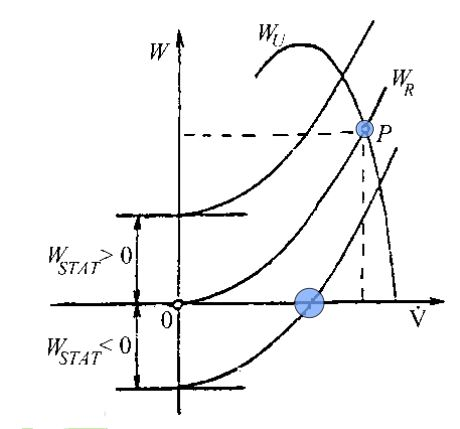
\includegraphics[width=0.4\textwidth]{figures/carac_pompe_circuit.png}
	\caption{Courbes caractéristiques pompe-circuit}
	\label{fig:carac_pompe_circuit}
\end{figure}

\subsection{Expliquez la compression bi-étagée par rapport à la compression mono-étagée.}
Lorsque l'on comprime avec un seul étage, la température peut monter très haut. Par conséquent, des matériaux résistants à de grandes températures doivent être utilisés, ce qui coûte plus cher. Le travail moteur nécessaire à la compression sera minimum pour une compression avec une infinité d'étages donnant lieu, théoriquement, à une compression isotherme. Pour des raisons de place et de budget, un équilibre est généralement trouvé pour le nombre d'étages. 

La compression bi-étagée offre aussi la possibilité d'insérer une refroidissment entre les deux compresseurs, permettant ainsi d'atteindre des ratios de compression plus importants.

\subsection{À partir de la droite d'Euler, comment obtenir la courbe caractéristique ? \label{ssec:droiteEuler}}
La droite d'Euler est de la forme :
\begin{equation} W_m = u^2\left(1-\frac{\dot{V}}{\dot{V}_X}\right) \end{equation}
Les différentes dissipations imputables à l'écoulement du fluide sont :
\begin{itemize}
	\item L'écoulement du fluide dans le canal. On le modélise comme étant proportionnel au carré du débit volumique. $W_{fL} = K_L\dot{V}^2$;
	\item L'éventuel changement de direction brusque du fluide qui intervient à l'entrée du canal. On peut considérer que pour un certain débit, ces pertes seront nulles. On a donc $W_{f1} = K_1(\dot{V}-\dot{V}_Y)^2$;
	\item De même pour l'éventuel changement de direction à la sortie du canal. On a donc $W_{f2} = K_2(\dot{V}-\dot{V}_Z)^2$.
\end{itemize}
En sommant les différentes contributions, on obtient les courbes de la Figure \ref{fig:droiteEuler}.
\begin{figure}[h]\centering
	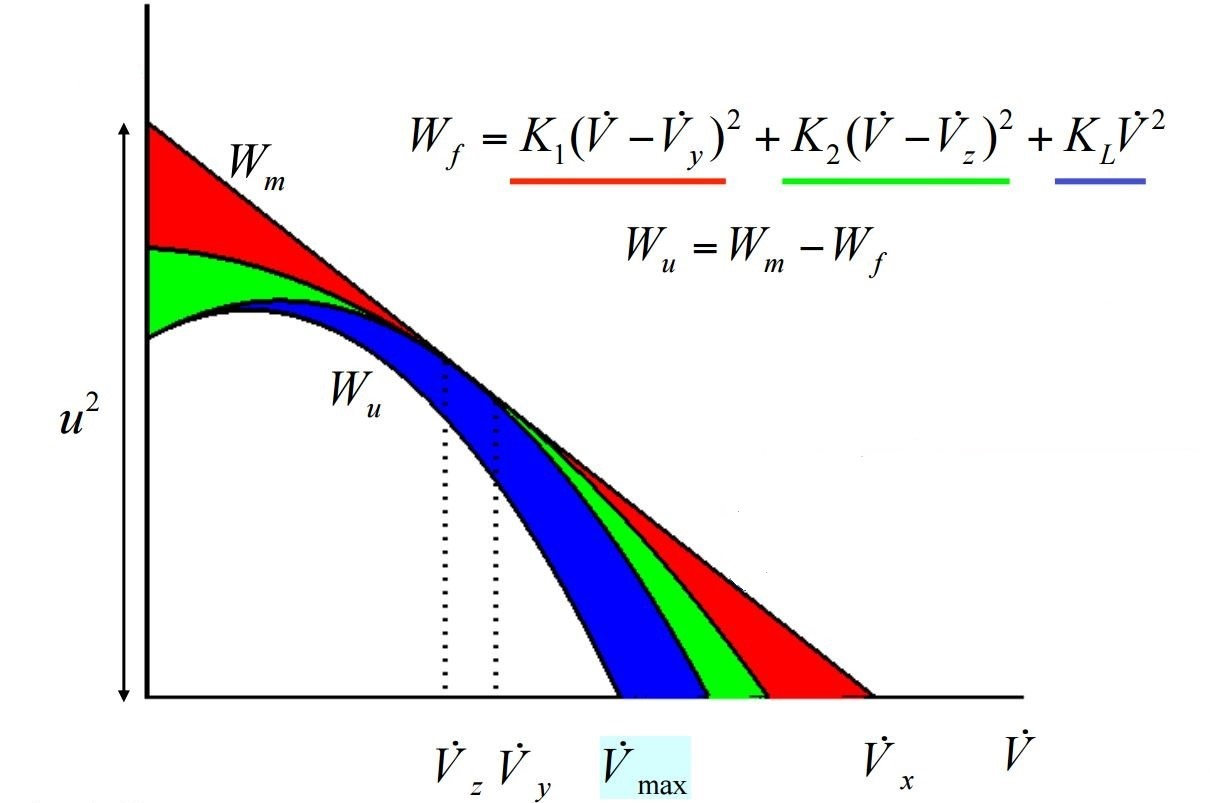
\includegraphics[width=0.6\textwidth]{figures/courbescaracteristiques.png}
	\caption{Courbes caractéristiques}
	\label{fig:droiteEuler}
\end{figure}

\subsection{Démontrez, pour une machine radiale, l'expression de la droite d'Euler à partir de l'équation générale \ref{eq:eulergenerale}.}
\begin{equation} W_m = u_2c_2\cos(\alpha_2)-u_1c_1\cos(\alpha_1) \label{eq:eulergenerale} \end{equation}
Pour une machine radiale, $\alpha_1 = \SI{90}{\degree}$. On a donc 
\begin{equation} W_m = u_2c_2\cos(\alpha_2) \end{equation} 
On peut trouver par le triangle des vitesses l'expression suivante
\begin{equation} c_2\cos(\alpha_2) = u_2-c_{2r}\tan(\beta_2) \end{equation}.
En posant $\dot{V} = 2\pi b_2r_2c_{2r}$ on trouve :
\begin{equation} \frac{W_m}{u_2^2} = 1 - \dot{V}\frac{\tan(\beta_2)}{2\pi b_2r_2u_2} \end{equation}

\subsection{Définissez les grandeurs physiques de la droite d'Euler, les pertes à prendre en compte pour obtenir une relation plus correcte. Justifiez physiquement la présence de ces pertes. Représentez la courbe obtenue avec ces pertes et la droite sur un même schéma. Comment obtenir en pratique le point de fonctionnement correspondant à l'intersection de la droite avec l'axe des abscisses ?}
La réponse à la droite d'Euler est disponible à la question \ref{ssec:droiteEuler} et la réponse concernant le point de fonctionnement à la question \ref{ssec:caracpompecircuit}.

\subsection{Dessinez le diagramme TS d'une compression polytropique. Identifiez les surfaces représentant le travail isentropique.}
Voir Figure \ref{fig:compressionpolytropique}.
\begin{figure}[h]\centering
	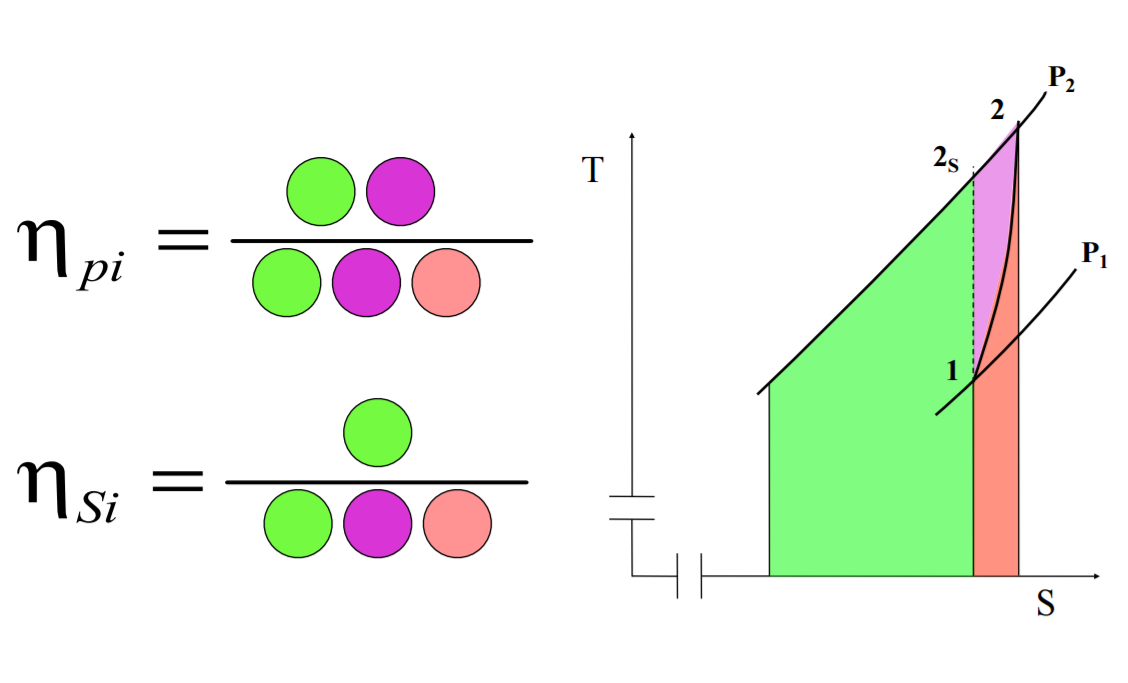
\includegraphics[width=0.7\textwidth]{figures/compressionpolytropique.png}
	\caption{Compression polytropique}
	\label{fig:compressionpolytropique}
\end{figure}

\subsection{Expliquez ce qu'il se passe quand on essaie de pompe de l'eau dans un puits de \SI{12}{\meter} plus bas que le niveau de la pompe à pression atmosphérique. Expliquez comment résoudre ce problème et la condition à respecter de manière générale.}
Pour aspirer l’eau dans un puits situé 12m plus bas que le niveau de la pompe, il faudrait une dépression en haut de la colonne d’eau au moins égale à la pression (générée par le poids de l’eau) en bas de la colonne d’eau. Plus la colonne est haute, plus cette dépression doit être importante. Or, lorsque la pression d’un liquide descend sous la valeur de la pression de vapeur, le liquide se vaporise. Ce phénomène est très dangereux à l’intérieur d’une pompe centrifuge car il crée une cavitation (implosion de bulles de vapeur) qui endommage le corps de pompe tout en réduisant le rendement. 
La hauteur d’eau à l’aspiration limite donc la dépression qu’il est possible de créer sans que l’eau se vaporise. Si la hauteur d’eau est trop importante pour être soulevée sans se vaporiser, il faudra placer des pompes intermédiaires.

\subsection{Comparez sur graphe TS une compression isotherme et une compression standard.}
Une compression standard demandera un travail moteur nettement plus grand qu'une compression isotherme. En effet, la compression isotherme requiert un minimum de travail. On peut arriver à une compression isotherme en ayant une infinité d'étages.
\begin{figure}[h]\centering
	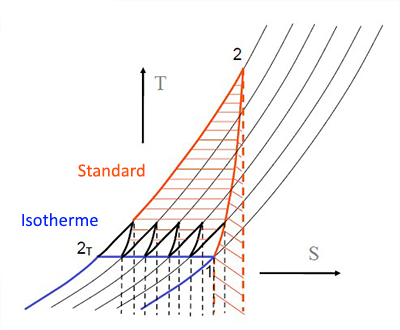
\includegraphics[width=0.6\textwidth]{figures/compisotherme.png}
	\caption{Compression isotherme et standard}
\end{figure}
